%!TEX root =  main.tex
%The sensors are differentiated in terms of their prediction efficiency and cost. 



A learner has access to $K\geq 2$ sensors that provide predictions
of an unknown label. \todoc{We agreed with Venkatesh, that in the intro, he will explain that
the classifiers themselves are a kind of intelligent sensors. So the sensors mentioned here
are really the classifiers themselves. ``Intelligent, super-sensors''.
The advantage of talking about sensors only is that we don't really care about what 
goes into the classifiers anyways.
}
 It is assumed that the sensors form a cascade (cf. \cref{wrap-fig:1}),
i.e., they are  \emph{ordered} in terms of their prediction efficiency,
later sensors are more accurate in predicting the unknown label.
However, acquiring the output of later sensor comes at a fixed cost.
The dilemma of the learner is that while he knows the ordering of the sensors,
the accuracies of the sensors are unknown.
The learner's task is to minimize the total prediction cost, which includes
both the cost of acquiring the sensor outputs and the cost incurred due to imperfect
sensor output.
The learner knows the costs, but does not know how efficient the sensors are
and learns only the output of the sensors.
Learning happens in a sequential setting, where in each round the learner can decide
sequentially (within the round) which sensor outputs to observe,
while respecting the ordering of the sensors.
The output of the last sensor selected serves as the prediction for the round.


\begin{wrapfigure}{r}{5cm}
	\vspace{-.5cm}
	\centering
	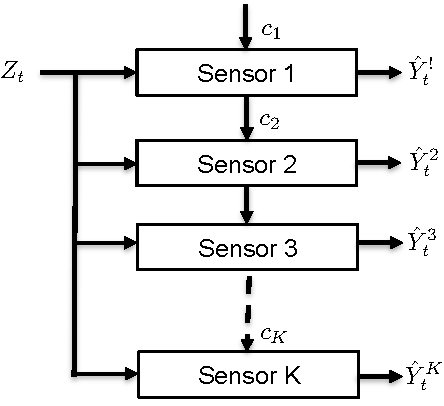
\includegraphics[scale=.6]{../Figures/SensorCascade}
	\caption{Cascade of sensors.
	Each sensor predicts a label $Y_t$ (not shown) associated
	with a random instance $Z_t$. The output of sensor $k$
	can be acquired at the additional cost $c_{k-1}>0$ after 
	the output of sensor has been acquired. Sensors with higher indices
	have a smaller probability of missing the true label.
	}\label{wrap-fig:1}
	\vspace{-.5cm}
\end{wrapfigure} 


The formal specification of the learning problem is as follows:
Learning happens sequentially.
In round $t$ ($t=1,2,\dots$), 
the environment generates 
$(Y_t,\hY_t^1,\dots,\hY_t^K)\in \{0,1\}^{K+1}$ from a distribution $P$ unknown to the learner.
\todoc{Do we use anywhere that labels are binary? If not, why not present a general case?}
Here, $Y_t$ is the unknown label 
%of context/instance $Z_t$ to be predicted
 in round $t$, while $\hY_t^k$ is the output of sensor
$k$, a prediction of $Y_t$. 
%We focus on the case where $Z_t$ is not available to the learner. 
%The case where they are observed is briefly discussed in the supplementary. 
At the cost of $c_1+ c_2 + \dots + c_k$,
the learner can choose to acquire the outputs of the first $k$ sensors,
where $k\in [K] := \{1,\dots,K\}$. 
\todoc{Now, here we are not talking about acquiring the sensor outputs in a sequential fashion.
Do we need to modify the introduction where we promised that this will happen? 
Can we justify why won't consider the fully sequential case? For simplicity?
In fact, if we did consider the fully sequential case 
then the natural action space would be more complicated:
The actions would be trees, describing the policies of when to continue to acquire new sensors. 
}
Here, $c_i\ge 0$ is the marginal cost of acquiring the output of sensor $i$.
The costs $c := (c_1,\dots,c_K)$ are known to the learner.
Having acquired the output of the first $k$ sensors, the learner predicts the unknown label $Y_t$ using
the output of the last sensor acquired, i.e., using $\hY_t^k$, making the learner incur the loss
\begin{align*}
L_t(k)=\mathbf{1}_{\{\hat{Y}^k_t\neq Y_t\}}+\sum_{j=1}^k c_j\,
\end{align*}
in round $t$.
The feedback of learner for this round is then $H_t(k)=(\hat{Y}^1_t,\ldots,\hat{Y}^k_t)$.

%Let $\{Z_t, Y_t\}_{{t>0}}$ denote a sequence generated according to an unknown distribution. $Z_t \in\mathcal{C} \subset  \mathcal{R}^d$, where $\mathcal{C}$ is a compact set, denotes a feature vector/context at time $t$ and $Y_t \in \{0,1\}$ its binary label. We denote output/prediction of the $i^{th}$ sensor as $\hat{Y}^i_t$ when its input is $Z_t$. The set of actions available to the learner is $\mathcal{A}=\{1,\ldots, K\}$, where  the action $k \in \mathcal{A}$ indicates acquiring predictions from sensors $1,\ldots, k$ and classifying using the prediction $\hat{Y}^k_t$. 

\if0
The prediction error rate of the $i^{th}$ sensor is denoted as $\gamma_i:=\Pr\{Y_t\neq \hat{Y}^k_t\}$. The learner incurs an extra cost of $c_k\geq 0$ to acquire output of sensor $k$ after acquiring output of sensor $k-1$. The sensor cascade is depicted in the adjacent figure. In this section we assume that the error rate does not depend on the  context, and the treatment with contextual information is given in the supplementary. 
\fi

%Let $H_t(k)$ denote the feedback observed in round $t$ from action $k$. Since we observe predictions of all the first $k$ senors by playing action $k$, we get   $H_t(k)=(\hat{Y}^1_t,\ldots,\hat{Y}^k_t)$.
%The loss incurred in each round is defined in terms of the prediction error and the total cost involved. When the learner selects action $k$, loss is the prediction error of sensor $k$ plus sum of the costs incurred along the path ($c_1,\ldots,c_k$). Let $L_t: \mathcal{A}\rightarrow \mathcal{R}_+$ denote the loss function in round $t$. Then,
%\begin{equation}
%L_t(k)=\mathbf{1}_{\{\hat{Y}^k_t\neq Y_t\}}+\sum_{j=1}^k c_j.
%\end{equation} 
We refer to the above setup as Sensor Acquisition Problem (SAP).
Based on the previous description, an instance of SAP is the tuple $\psi = (K,P,c)$, where $K\in \mathbb{N}$, $K\ge 2$,
$P$ is a distribution over $\{0,1\}^{K+1}$ and $c\in [0,\infty)^K$. \todoc{I got rid of $c_0$.}
 A policy $\pi$ on a $K$-sensor SAP problem
 is a sequence of maps, $(\pi_1, \pi_2, \cdots)$, where
 $\pi_t : \mathcal{H}_{t-1}\rightarrow [K]$ gives the action selected in round $t$
 given a history $h_{t-1}\in \mathcal{H}_{t-1}$ that consists of all actions and corresponding feedback observed before $t$. 
 Let $\Pi$ denote set of such policies. 
 For any $\pi \in \Pi$, we compare its performance to that of the single best action in hindsight 
 and define its expected regret as follows
\begin{equation}
R^\psi_T(\pi)= \mathbb{E}\left[\sum_{t=1}^T L_t(I_t)\right]-\min_{k\in A}\mathbb{E}\left[\sum_{t=1}^T L_t(k)\right],
\end{equation}
where $I_t$ denotes the action selected by $\pi_t$ in round $t$.
\todoc{I prefer upper case for random variables. Also, later the paper is quite inconsistent in its notation for actions. Sometimes we have $i_s$, $A_t$, then $a_t$, etc. This should be unified.}
The goal of the learner is to learn a policy that minimizes the expected total loss, or, equivalently, to minimize the expected regret, i.e.,
\begin{equation}
\pi^*= \arg \min_{\pi \in \Pi } R^\psi_T(\pi).
\end{equation}

\noindent
{\bf Optimal action in hindsight: } For any $t$, we have 
\begin{equation}
\label{eqn:OptimalAction}
\mathbb{E}[L_t(k)]=\Pr\{Y_t\neq \hat{Y}^k_t\}+\sum_{j=1}^kc_j=\gamma_k +\sum_{j=1}^k c_j\,,
\end{equation}
where $\gamma_k=\Pr\{Y_t\neq \hat{Y}^k_t\}$ is the misclassification error rate of sensor $k$.
Let $k^*=\arg\min_{k\in [K]} \gamma_k + \sum_{i\le  k}c_i$. \todoc{I got rid of $\mathcal{A}$. Let's instead use $[K]$. Simpler. Fewer symbols. Also, for some reason we had $\sum_{i<k}$. I fixed this.}
Then the optimal policy is to play action $k^*$ in each round. 
If an action $i$ is played in any round then it adds $\Delta_k:=\gamma_k + \sum_{i\le k}c_i -( \gamma_{k^*} + \sum_{i\le k^*}c_i)$ to the expected regret. 
Let $N_k(s)$ denote the number of times action $k$ 
is selected till time $s$, i.e., $N_k(s)=\sum_{t=1}^s \boldsymbol{1}_{\{I_t=k\}}$. 
Then the expected regret can be expressed as \todoc{Why do we have this here? Add explanation or remove this.}
\begin{eqnarray}
\label{eqn:ExpRegretGap}
R^\psi_T(\pi)&=& \sum_{k \in [K]}\mathbb{E}[N_k(T)]\Delta_k\,.
\end{eqnarray}\

